\documentclass[]{minimal}
\usepackage{tikz}
\usetikzlibrary{positioning}
\usetikzlibrary{arrows}
\usetikzlibrary{patterns}

\begin{document}

\pagestyle{empty}

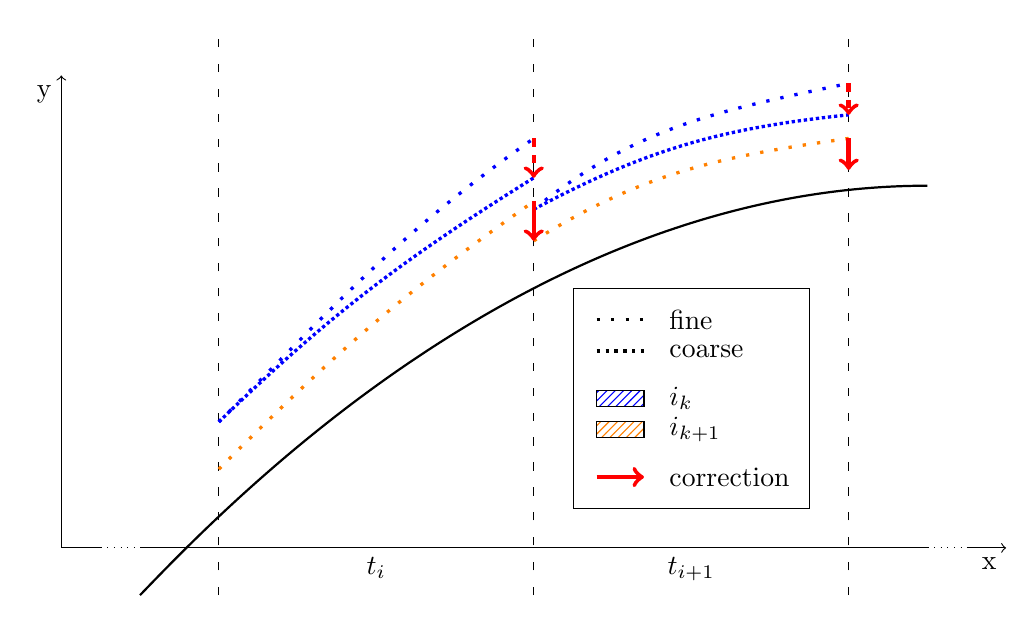
\begin{tikzpicture}[scale=2]


% coordinates
\draw[->] (0,0) -- (0,3) node[pos=1,below left] {y};

\draw[-] (0,0) -- (.25,0);
\draw[dotted] (.25,0) -- (.5,0);
\draw[-] (.5,0) -- (5.5,0);
\draw[dotted] (5.5,0) -- (5.75,0);
\draw[->] (5.75,0) -- (6,0) node[pos=1,below left] {x};

% threads
\draw[loosely dashed] (1,-.3) -- (1,3.3);
\draw[loosely dashed] (3,-.3) -- (3,3.3);
\draw[loosely dashed] (5,-.3) -- (5,3.3);
\node[below] at (2,0) {$t_{i}$};
\node[below] at (4,0) {$t_{i+1}$};

% exact
\draw[thick] (.5,-.3) parabola  bend +(5,2.6) (5.5,2.3);

\begin{scope}[very thick]

% pCoarse
\begin{scope}[loosely dotted, color=blue]
\draw (1,.8) to[out=45,in=215] (3,2.6);
\draw (3,2.15) to[out=39,in=192] (5,2.95);
\end{scope}

% pFine
\begin{scope}[densely dotted, color=blue]
\draw (1,.8) to[out=44,in=212] (3,2.35);
\draw (3,2.15) to[out=28,in=186] (5,2.75);
\end{scope}

% coarse
\begin{scope}[loosely dotted, color=orange]
\draw (1,.5) to[out=45,in=215] (3,2.2);
\draw (3,1.95) to[out=32,in=188] (5,2.6);
\end{scope}
\end{scope}

% merges
\begin{scope}[red, ultra thick]
\draw[->] (3,2.2) -- (3,1.95);
\draw[->, dashed] (3,2.6) -- (3,2.35);

\draw[->] (5,2.6) -- (5,2.4);
\draw[->, dashed] (5,2.95) -- (5,2.75);
\end{scope}

%legend
\draw[] (3.25,.25) rectangle (4.75, 1.65);

\begin{scope}[anchor=west]
    \node[] at (3.8,1.45) {fine};
    \node[] at (3.8,1.25) {coarse};
    \node[] at (3.8,.95) {$i_k$};
    \node[] at (3.8,.75) {$i_{k+1}$};
    \node[] at (3.8,.45) {correction};
\end{scope}

\draw[-, loosely dotted,very thick] (3.4,1.45) -- (3.7,1.45);
\draw[-, dotted,very thick] (3.4,1.25) -- (3.7,1.25);
\draw[pattern color=blue,pattern=north east lines] (3.4,.9) rectangle (3.7, 1);
\draw[pattern color=orange,pattern=north east lines] (3.4,.7) rectangle (3.7, .8);
\draw[->,red, ultra thick] (3.4,.45) -- (3.7,.45);

\end{tikzpicture}

\end{document}